\section{Einf�hrung in GIT}
\subsection{Dezentrale Versionierung}
\begin{frame}
  \frametitle{Dezentrale Versionierung}
  \tableofcontents[currentsection,currentsubsection]
\end{frame}
\begin{frame}
  \frametitle{Dezentrale Versionierung}
  \begin{itemize}
    \item<1->Kopie des Repositorys in jeder Arbeitskopie enthalten
      \begin{itemize}
        \item In: \texttt{<project-path>/.git}
        \item Arbeitskopie und Repository synonym
      \end{itemize}
    \item<2->Import und Export zwischen Repositories
      \begin{itemize}
          \item zentrale Repositories zur Zusammenarbeit m�glich
          \item Unterscheidung lokale und entfernte Repositories ("`Remotes"')
      \end{itemize}
    \item <3->Fast s�mtliche Versionierungsarbeit im lokalen Repository
      \begin{itemize}
          \item Wesentlich h�here Arbeitsgeschwindigkeit
      \end{itemize}
    \item <4->Freiheit f�r die Entwickler
  \end{itemize}
\end{frame}
\subsection[Trees, Commits \& Blobs]{Aufbau und Bestandteile von GIT-Repositories}
\begin{frame}
  \frametitle{Trees, Commits \& Blobs}
  \tableofcontents[currentsection,currentsubsection]
\end{frame}
\begin{frame}
  \frametitle{Trees, Commits \& Blobs}
  \begin{itemize}
    \item Jede Version in Objektdatenbank in \texttt{.git/objects}
    \item <2->Blob-Objekte
      \begin{itemize}
        \item Datei-Inhalte
      \end{itemize}
    \item <3->Tree-Objekte
      \begin{itemize}
        \item Verzeichnisse
      \end{itemize}
    \item <4->Commit-Objekte
      \begin{itemize}
        \item Tree-Snapshots
      \end{itemize}
  \end{itemize}
\end{frame}
\begin{frame}
  \frametitle{Blob-Objekte}
  \begin{itemize}
    \item Repr�sentieren Inhalte (von Dateien)
    \item Dargestellt durch einen SHA1-Hashwert (u.A. abh�ngig vom Inhalt der Datei)
    \item Gleicher Datei-Inhalt $\Rightarrow$ Wiederverwendung des Blob-Objekts
    \item Kein Blob-Objekt, keine Versionierung
      \begin{itemize}
        \item Leere Verzeichnisse werden nicht versioniert.
      \end{itemize}
  \end{itemize}
\end{frame}
\begin{frame}
  \frametitle{Tree-Objekte}
  \begin{itemize}
    \item<1>Entsprechen Verzeichnissen im Dateisystem
    \item<1>Ebenfalls durch SHA1-Hashwert dargestellt
      \begin{itemize}
        \item unter Anderem abh�ngig von den enthaltenen Trees und Blobs
      \end{itemize}
    \item<1>Mindestens ein Blob- oder Tree-Objekt inklusive Namen zugeordnet
      \begin{itemize}
        \item Tree und Blob oder anderer Tree ergeben Datei-/Verzeichnisreferenz
      \end{itemize}
  \end{itemize}
\end{frame}
\begin{frame}
  \frametitle{Tree-Objekte Beispiel}
  \begin{center}
    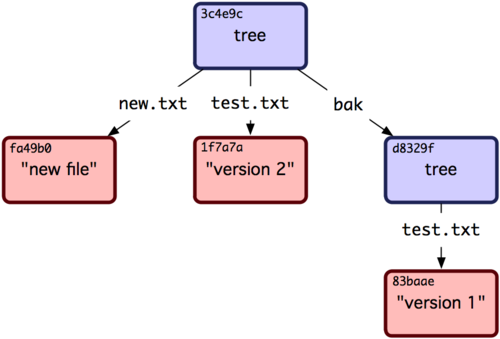
\includegraphics{images/tree-example.png}
  \end{center}
\end{frame}
\begin{frame}
  \frametitle{Commit-Objekte}
  \begin{itemize}
    \item<1->Speichern Versionen der Daten
    \item<1->Beinhalten ein Tree-Objekt und einen oder mehrere Eltern-Commits
    \item<1->Dargestellt durch SHA1-Hashwert ($=$ Commit-ID)
      \begin{itemize}
        \item unter Anderem abh�ngig von den enthaltenen Trees, dem Autor sowie dem Datum und der Uhrzeit des Commits
      \end{itemize}
    \item<2->Commit-ID abh�ngig von den Trees $\Rightarrow$ abh�ngig von den Blobs $\Rightarrow$ abh�ngig von den Datei-Inhalten
    \item<3->Commit in Gesamtheit als \emph{Arbeitsschritt $X$} zum
      \emph{Zeitpunkt $Y$} von \emph{Person $Z$} global eindeutig identifizierbar
    \item<4->(Sicherheits-)kopie aller Commits in jeder Arbeitskopie vorhanden
    \item<5->$\Rightarrow$ Sicherheitsvorteil (bsp. Linux Kernel)
  \end{itemize}
\end{frame}
\begin{frame}
  \frametitle{Commit-Objekte Beispiel}
  \begin{center}
    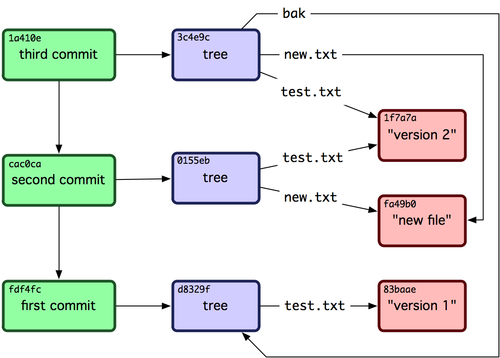
\includegraphics{images/commit-example.png}
  \end{center}
\end{frame}
\subsection[Remotes, Branches \& Tags]{Verteilung und Strukturierung der Historie}
\begin{frame}
  \frametitle{Remotes, Branches \& Tags}
  \tableofcontents[currentsection,currentsubsection]
\end{frame}
\begin{frame}
  \frametitle{Remotes, Branches \& Tags}
  \begin{itemize}
    \item Verteilung und Organisation des Commit-Trees
    \item<2->Remotes
      \begin{itemize}
        \item Entfernte Repositories zur gemeinsamen Verwendung
        \item Verwaltung mehrerer Remotes m�glich
      \end{itemize}
    \item<3->Branches \& Tags
      \begin{itemize}
        \item Organisation verschiedener Entwicklungszweige und Releases.
      \end{itemize}
  \end{itemize}
\end{frame}
\begin{frame}
  \frametitle{Remotes}
  \begin{itemize}
    \item Dienen der Verteilung der Commits und Branches
    \item<2->Lokal oder irgendwo im Netzwerk/internet
    \item<3->Verschiedene Deployment- und Entwicklungsremotes m�glich
    \item<4->Bonus: SVN-Remotes ebenfalls m�glich
      \begin{itemize}
        \item Killer-Methode zur Migration von SVN zu GIT
        \item Ansonsten aufgrund der Implementierungsdetails nur in wenigen F�llen praktikabel
      \end{itemize}
    \item<5->Vorgriff: Zur Verteilung von Commits ist ein Schritt mehr erforderlich als bei SVN.
      \begin{itemize}
        \item<6->ABER: It's a feature, not a constraint.
      \end{itemize}
  \end{itemize}
\end{frame}
\begin{frame}
  \frametitle{Branches \& Tags}
  \begin{itemize}
    \item<1->Branches und Tags sind \textbf{keine} Kopien von Unterverzeichnissen in andere Unterverzeichnisse innerhalb des Repositorys sondern \textbf{Referenzen auf Objekte}.
      \begin{itemize}
        \item Ausgereifter Branching-Mechanismus im VCS implementiert und nicht durch den Entwickler emuliert
      \end{itemize}
    \item<2->Referenzieren meistens Commits
    \item<3->Elterncommits werden dem Branch/Tag zugeordnet
    \item<4->Branch-Referenzen zeigen immer auf den neuesten Commit, Tags sind konstant (meistens)
    \item<5->Unterscheidung zwischen Remote und Lokalen Branches
      \begin{itemize}
        \item \texttt{origin/master} und \texttt{master} verschiedene Branches
      \end{itemize}
  \end{itemize}
\end{frame}
\begin{frame}
  \frametitle{Branches Beispiel}
  \begin{center}
    \vspace{-1cm}
    \begin{tabular}{p{0.55\textwidth}p{0.35\textwidth}}
      \center{\textbf{Vorher}} & \center{\textbf{Nachher}} \\
      \vspace{-8mm}\begin{FlushLeft}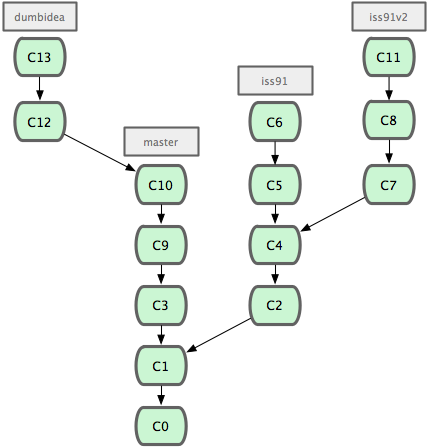
\includegraphics[height=.75\textheight]{images/branch-example.png}\end{FlushLeft} &
      \vspace{-8mm}\begin{flushright}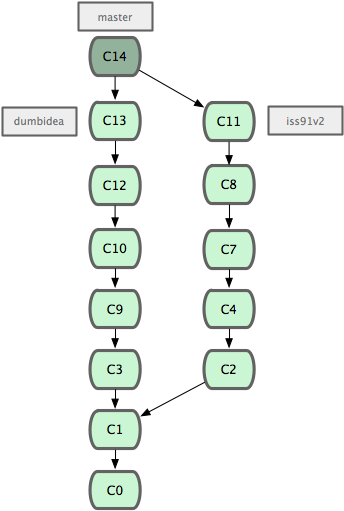
\includegraphics[height=.75\textheight]{images/branch-example2.png}\end{flushright}\\
    \end{tabular}
  \end{center}
\end{frame}
